\documentclass{beamer}

%-----------------------
%% This template is based on a template developed by the SMCS
%% (Statistical Methodology and Computing Service) at UCLouvain

%-----------------------
% pour faire les slides papiers :
% \documentclass[handout, compress]{beamer}
% \usepackage{pgfpages}
% % 4 par page
% \pgfpagesuselayout{4 on 1}[a4paper,border shrink=5mm, landscape]
% % 2 par page
% \pgfpagesuselayout{2 on 1}[a4paper,border shrink=5mm]

\usetheme{UCL2018}

\usepackage[utf8]{inputenc}
\usepackage[T1]{fontenc}
\usepackage{lmodern}
\usepackage{xspace}
\usepackage{float}
\usepackage{graphicx}
\usepackage{amssymb}
\usepackage{hyperref}
\usepackage{ragged2e}
\usepackage[authoryear, round]{natbib}

%% For slides in French
%% \usepackage[french]{babel}
%% \usepackage[cyr]{aeguill}

\usepackage{lipsum}

\theoremstyle{example}
\newtheorem{examplef}{Example}
\newtheorem{examplesf}{Examples}
\newcommand{\ei}{\end{itemize}}

\usepackage{xmpincl}


\title{Probabilistic mapping  of the sub-cellular proteome}
\author[]{Laurent Gatto}
\date{\today}
\institute[]{CBIO, de Duve Institute, UCLouvain}


\begin{document}

\pdfinfo {/Author(Laurent Gatto - UCLouvain)}


%-----------------------------------------------
% Title page
%-----------------------------------------------

\begin{frame}[plain]
\titlepage
\end{frame}


\begin{frame}%[noframenumbering]
%\thispagestyle{empty}

% Logo UCL a gauche
%% \begin{tikzpicture}
%%   \useasboundingbox (0,0) rectangle(\the\paperwidth,1);
%%   \node[inner sep=0pt] at (1.7,.5) {
\includegraphics[width=.33\textwidth]{UCL_2018}};
%%  \end{tikzpicture}

\justify

{\small \textbf{Abstract:} In biology, localisation is function -
  understanding the sub-cellular localisation of proteins is paramount
  to comprehend the context and full extend of their
  functions. Shotgun mass spectrometry-based spatial proteomics method
  are orthogonal to widely used targeted microscopy-based assay. In
  conjunction with contemporary machine learning, the former enable to
  build proteome-wide protein localisation maps, informing us on the
  location of thousands of proteins. When studying these proteome-wide
  spatial maps, one can learn that while some proteins can be found in
  a single location within a cell, up to half of the proteins may
  reside in multiple locations, can dynamically re-localise, or reside
  within an unknown functional compartment, leading to considerable
  uncertainty in associating proteins to their sub-cellular
  location. Recent Bayesian modelling approaches enable us to mine
  these data, and in particular the dynamic fraction of the spatial
  proteome, in much greater depth. We are now in a position to (1)
  probabilistically model protein localisation as well as quantify the
  uncertainty in the location assignments, and (2) compute a
  probability for, and quantify uncertainty in, whether a protein is
  differentially localised upon cellular perturbation. These
  computational approaches lead to better and more trustworthy
  biological interpretation of these rich spatial proteomics data.  }


\end{frame}


\begin{frame}{Acknowledgements}

  \begin{itemize}

  \item \textcolor{Blue}{Mr Oliver Crook}

  \item \textcolor{Blue}{Dr Lisa Breckels}

  \end{itemize}


\end{frame}


%-----------------------------------------------
% Table of content
%-----------------------------------------------

\AtBeginSection[]{
  \setbeamercolor{background canvas}{bg=UCLblue2}
  \setbeamercolor{section in toc}{fg=UCLblue}
  \setbeamercolor{subsection in toc}{fg=UCLblue}
  \setbeamerfont{section in toc}{size=\large}

  \mode<handout>{
    \setbeamercolor{background canvas}{bg=white}
    \setbeamercolor{section in toc}{fg=UCLblue}
    \setbeamercolor{subsection in toc}{fg=UCLblue}
  }

  \begin{frame}[plain]
    \frametitle{Outline}
    \tableofcontents[currentsection,hideothersubsections]
  \end{frame}

  \setbeamercolor{background canvas}{bg=white}
}


%-----------------------------------------------
% Content
%-----------------------------------------------

\section{Spatial proteomics}


\begin{frame}{Cell organisation - \textbf{localisation is function}}
  \begin{center}
    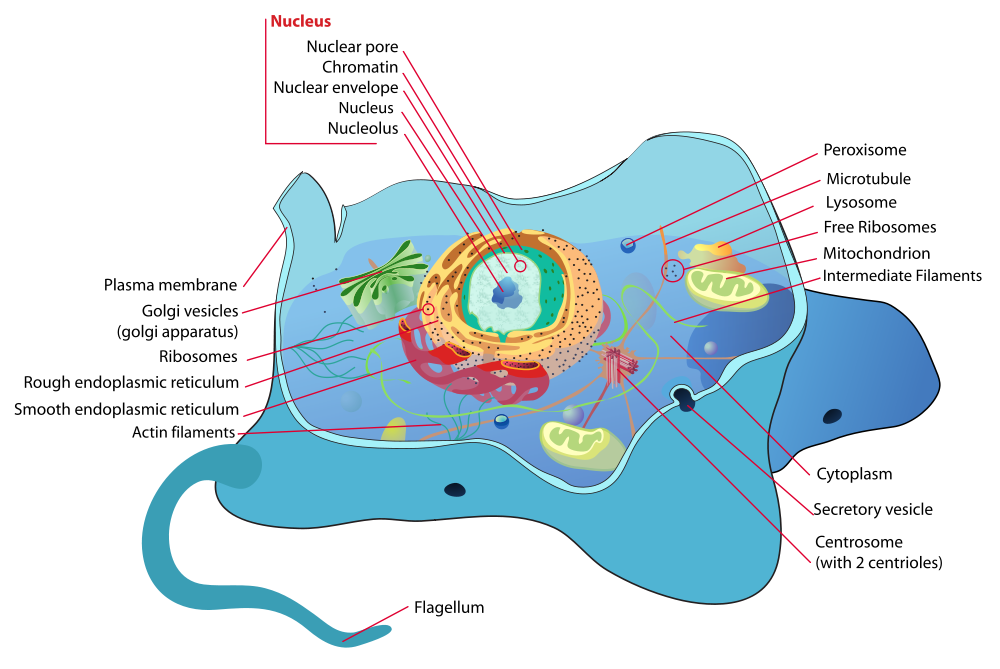
\includegraphics[width=.8\linewidth]{figs/Animal_cell_structure.png} \\
    \textbf{\textcolor{Blue}{Spatial proteomics}} is the systematic
    study of protein localisations.
  \end{center}

  \begin{center}
    \textbf{Localisation -- re-localisation -- mis-localisation}
  \end{center}
  
  \tiny Image from Wikipedia
  \url{http://en.wikipedia.org/wiki/Cell_(biology)}.  
\end{frame}


\begin{frame}{}

  \begin{columns}
    \begin{column}{0.5\textwidth}

      \textbf{Explorative/discovery approaches},
      \textcolor{Blue}{steady-state \textbf{global localisation maps}}
      (as opposed to microscopy-based targeted approaches).

      \bigskip
      
      \small{

        \textbf{Density gradient}: PCP \citep{Dunkley:2006}, LOPIT
        \citep{Foster2006}, hyperLOPIT
        \citep{Christoforou:2016,Mulvey:2017} and \\

        \textbf{Differential centrifugation} \cite{Itzhak:2016},
        LOPIT-DC \citep{Geladaki:2018}.

      }
     
      \bigskip
      
      
    \end{column}
    \begin{column}{0.5\textwidth}
      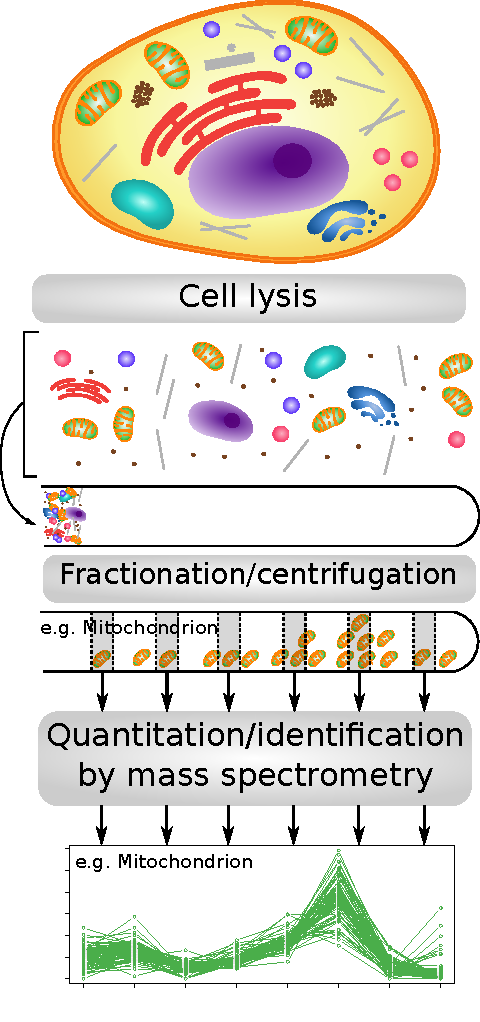
\includegraphics[width=.78\linewidth]{figs/workflow_primary.pdf}
    \end{column}    
  \end{columns}
  
\end{frame}

\subsubsection*{The data}
\label{sec:data}

\begin{frame}{Quantitation data}
  \begin{center}
    \begin{tabular}{|l|llll|}
      \hline
      & Fraction$_{\text{1}}$ & Fraction$_{\text{2}}$ & \ldots{} & Fraction$_{\text{L}}$ \\
      \hline
      {\bf x}$_{\text{1}}$ & $x_{\text{1,1}}$ & $x_{\text{1,2}}$ & \ldots{} & $x_{\text{1,L}}$ \\
      {\bf x}$_{\text{2}}$ & $x_{\text{2,1}}$ & $x_{\text{2,2}}$ & \ldots{} & $x_{\text{2,L}}$ \\
      {\bf x}$_{\text{3}}$ & $x_{\text{3,1}}$ & $x_{\text{3,2}}$ & \ldots{} & $x_{\text{3,L}}$ \\
      \vdots & \vdots & \vdots & \vdots & \vdots \\
      {\bf x}$_{\text{i}}$ & $x_{\text{i,1}}$ & $x_{\text{i,2}}$ & \ldots{} & $x_{\text{i,L}}$ \\
      \vdots & \vdots & \vdots & \vdots & \vdots \\
      {\bf x}$_{\text{N}}$ & $x_{\text{N,1}}$ & $x_{\text{N,2}}$ & \ldots{} & $x_{\text{N, L}}$ \\
      \hline
    \end{tabular}
  \end{center}
\end{frame}

\begin{frame}{Quantitation data and organelle markers}
  \begin{center}
    \begin{tabular}{|l|llll||l|}
      \hline
      & Fraction$_{\text{1}}$ & Fraction$_{\text{2}}$ & \ldots{} & Fraction$_{\text{L}}$ & markers\\
      \hline
      {\bf x}$_{\text{1}}$ & $x_{\text{1,1}}$ & $x_{\text{1,2}}$ & \ldots{} & $x_{\text{1,L}}$ & unknown \\
      {\bf x}$_{\text{2}}$ & $x_{\text{2,1}}$ & $x_{\text{2,2}}$ & \ldots{} & $x_{\text{2,L}}$ & \textcolor{Red}{$loc_{1}$}\\
      {\bf x}$_{\text{3}}$ & $x_{\text{3,1}}$ & $x_{\text{3,2}}$ & \ldots{} & $x_{\text{3,L}}$ & unknown \\
      \vdots & \vdots & \vdots & \vdots & \vdots & \vdots \\
      {\bf x}$_{\text{i}}$ & $x_{\text{i,1}}$ & $x_{\text{i,2}}$ & \ldots{} & $x_{\text{i,L}}$ & \textcolor{Blue}{$loc_{k}$}\\
      \vdots & \vdots & \vdots & \vdots & \vdots & \vdots\\
      {\bf x}$_{\text{N}}$ & $x_{\text{N,1}}$ & $x_{\text{N,2}}$ & \ldots{} & $x_{\text{N, K}}$ & unknown \\
      \hline
    \end{tabular}
  \end{center}
\end{frame}


%-----------------------------------------------
% New section
%-----------------------------------------------

\section{Data analysis}


\begin{frame}{Visualisation}
  \begin{figure}
    \centering
    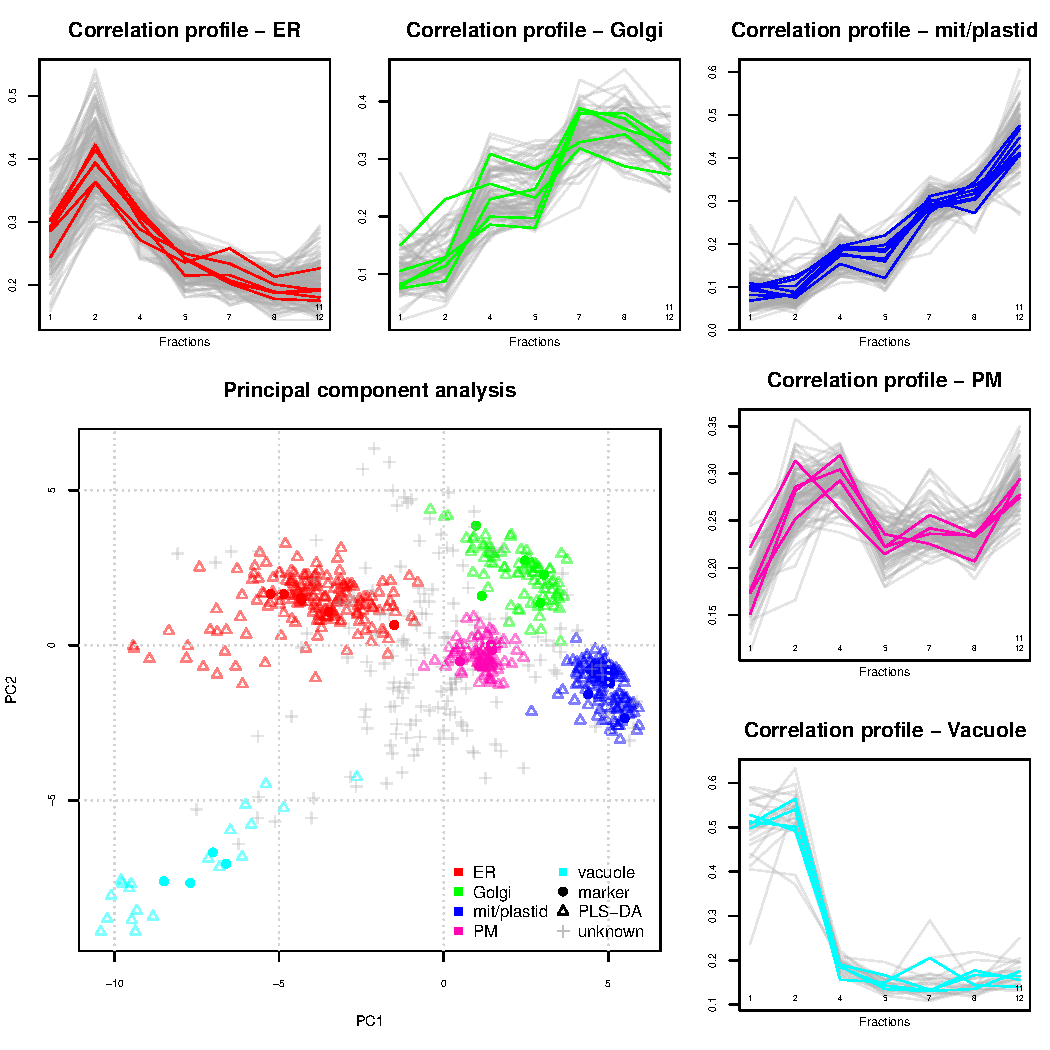
\includegraphics[width=.6\linewidth]{figs/F04-analyses.pdf}
    \caption{From \cite{Gatto:2010}, \textit{Arabidopsis thaliana} data
      from \cite{Dunkley:2006}}
  \end{figure}
\end{frame}

\subsubsection*{Machine learning}
\label{sec:ml}

\begin{frame}{Problem statement: classification}
  \begin{figure}[h]
    \centering
    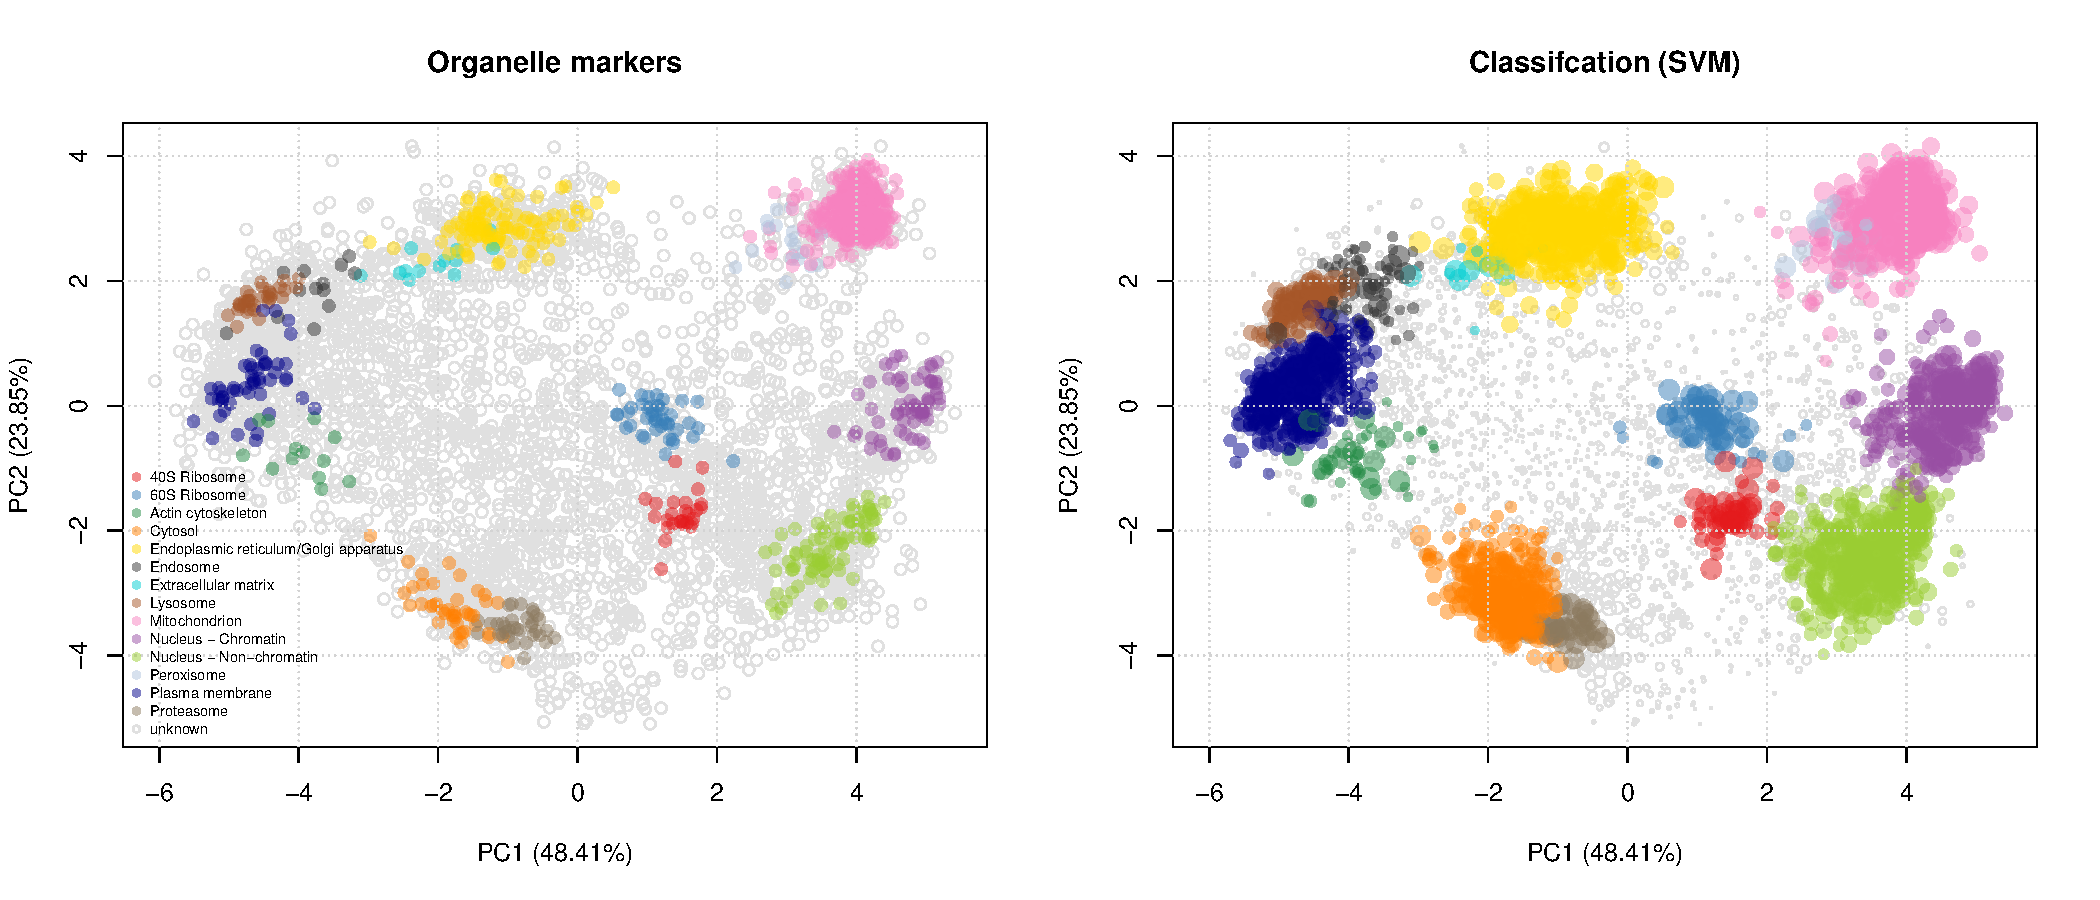
\includegraphics[width=\linewidth]{figs/hyperlopit-class.pdf}
    \caption{Support vector machines classifier (after 5\% FDR
      classification cutoff) on the embryonic stem cell data from
      \cite{Christoforou:2016}.}
  \end{figure}
\end{frame}

%-----------------------------------------------
% New section
%-----------------------------------------------

\section{Computational challenges}


\begin{frame}{Computational challenges}

  \begin{itemize}
  \item Visualisation (cluster, unsupervised learning)
  \item Classification (supervised learning)
  \item \textbf{Novelty detection} (semi-supervised learning)
  \item Data integration (transfer learning)
  \item \textbf{Unvertainty quantification}
  \item \textbf{Multi-localisation}
  \item \textbf{Spatial dynamics}
  \end{itemize}
  \centering

  \bigskip

  {\Large To uncover and understand biology}
\end{frame}


%-----------------------------------------------
% New section
%-----------------------------------------------

\section{Novelty detection}


\begin{frame}{Novelty detection}

\end{frame}


%-----------------------------------------------
% New section
%-----------------------------------------------

\section{Multi-localisation and uncertainly quantification}


\begin{frame}{Multi-localisation}

\end{frame}


%-----------------------------------------------
% New section
%-----------------------------------------------

\section{Spatial dynamics}


\begin{frame}{Spatial dynamics}

\end{frame}


%-----------------------------------------------
% New section
%-----------------------------------------------

\section{Behind the scences}


\begin{frame}{Behind the scences}

\end{frame}


%-----------------------------------------------
% References
%-----------------------------------------------


\begin{frame}[allowframebreaks]{References}
  \scriptsize
  \bibliographystyle{plainnat}
  \bibliography{refs}
\end{frame}


%-----------------------------------------------
% Final slide
%-----------------------------------------------

\begin{frame}%[noframenumbering]
%\thispagestyle{empty}

% Logo UCL a gauche
\begin{tikzpicture}
  \useasboundingbox (0,0) rectangle(\the\paperwidth,1);
  \node[inner sep=0pt] at (1.7,2) {
\includegraphics[width=.33\textwidth]{UCL_2018}};
 \end{tikzpicture}
\vspace{.1cm}



\begin{center}
  \textbf{Thank you for your attention}
\end{center}


\bigskip

Contact:

\begin{center}
  laurent.gatto@uclouvain.be – \url{lgatto.github.io/about}
\end{center}
 
\end{frame}


\end{document}
